%% latex_185_sharma_r.tex
%%
%% The following file is a skeleton file that demonstrates how to implement the IEEEtran.cls class 
%% file in LaTeX. This file is intended for the CMPE185 Technical Writing for Engineers Course in 
%% which the students must write a tutorial aimed towards novice LaTeX users in the LaTex environment.
%%
%% This file is heavily adapted from Michael Shell's bare_adv.tex file made available at 
%% http://www.ieee.org/conferences_events/conferences/publishing/templates.html
%%
%% You will need to rename this file with your information in the following format:
%% latex_185_last name_ first initial.tex
%% ---------------------------------------------------------------------------------------------------

% \documentclass{} precedes the preamble and is typically the first command in any .tex document. Every .tex document should include this command as it defines what kind of document you intend on creating. Modifiers in square brackets [] can be added in between the text ''documentclass'' and the curly brackets {} to modify font size, templates, etc. 

\documentclass[12pt,journal,compsoc]{IEEEtran}

%-----PACKAGES-------------------------------------------------------------------------------------

% Packages include extra commands that allow for additional formatting, ranging from Graphics, Math, to Alignment. The command to include packages will always look similar to \usepackage{} where the package name is within the curly brackets {}. Packages are defined in the preamble, i.e., between the \documentclass{} and \begin{document} commands.

% The following link takes you to a list of additional packages that may not be listed here. http://en.wikibooks.org/wiki/LaTeX/Package_Reference

% TO INCLUDE PACKAGES: 
% - Open the file ''latex_sample_packages.tex'' from the .zip folder.
% - From this file, COPY the code for the package you want to include and PASTE into your own .tex file.
% - Uncomment the package you want to include and load, i.e., remove the ''%'' in front of the \usepackage{package_name}.
 

% Copy package text here:
\usepackage{blindtext}
\usepackage{amsmath} 
\usepackage{graphicx}
\usepackage{balance}  
\usepackage{tikz}
\usepackage{inputenc}
\usepackage{caption}

% This is an example of how a \usepackage{} command should be included. You will need to include more packages to complete this assignment.




%----- The DOCUMENT Environment-------------------------------------------------------------------

% The \begin{document} and \end{document} commands establish the environment for the text of the document. The \begin{} and \end{} commands are used repeatedly in LaTeX to show where an environment begins and ends. The \end{document} command will be the last line of this .tex file.

\begin{document}

% The following commands are self explanatory. Insert your title, author and date into each command's curly bracket. You can include the abstract, paper header and paper footer information in this section then conclude the section with the command \maketitle (shown as the last line at the end of this section).

\title{LaTeX Tutorial for Beginners}
\author{Rakshya U Sharma}
% The double backslash \\ is used here to enter a ''Carriage Return'', or a line break. Note that the tilde ~ in between my name used as a ''Nonbreaking Space''. LaTeX will not break a structure at a ~ so this keeps an author's name from being broken across two lines. Also note that I included my name as an example so make sure to only insert your name in this command.

\date{\today}		% leaving the brackets empty omits the date
% To input the current date, you can type: \date{\today}

% The paper headers
%
% The only time the second header will appear is for the odd numbered pages
% after the title page when using the twoside option.
% 
% *** Note that you probably will NOT want to include the author's ***
% *** name in the headers of peer review papers.                   ***
% You can use \ifCLASSOPTIONpeerreview for conditional compilation here if
% you desire.

% The publisher's ID mark at the bottom of the page is less important with
% Computer Society journal papers as those publications place the marks
% outside of the main text columns and, therefore, unlike regular IEEE
% journals, the available text space is not reduced by their presence.
% If you want to put a publisher's ID mark on the page you can do it like
% this:
\IEEEpubid{0000--0000/00\$00.00~\copyright~2007 IEEE}
% or like this to get the Computer Society new two part style.
%\IEEEpubid{\makebox[\columnwidth]{\hfill 0000--0000/00/\$00.00~\copyright~2007 IEEE}%
%\hspace{\columnsep}\makebox[\columnwidth]{Published by the IEEE Computer Society\hfill}}
% Remember, if you use this you must call \IEEEpubidadjcol in the second
% column for its text to clear the IEEEpubid mark (Computer Society jorunal
% papers don't need this extra clearance.)


% use for special paper notices
%\IEEEspecialpapernotice{(Invited Paper)}

% for Computer Society papers, we must declare the abstract and index terms
% PRIOR to the title within the \IEEEcompsoctitleabstractindextext IEEEtran
% command as these need to go into the title area created by \maketitle.
\IEEEcompsoctitleabstractindextext{%
\begin{abstract}
%\boldmath
This document is a detailed tutorial on how to get started with LaTeX and design your document anyway you want. This tutorial is especially focused for beginners who have no background in LaTeX but it can also serve as a useful resource for people who already know how to use LaTeX. Lets Begin!!!!
\end{abstract}
% IEEEtran.cls defaults to using nonbold math in the Abstract.
% This preserves the distinction between vectors and scalars. However,
% if the journal you are submitting to favors bold math in the abstract,
% then you can use LaTeX's standard command \boldmath at the very start
% of the abstract to achieve this. Many IEEE journals frown on math
% in the abstract anyway. In particular, the Computer Society does
% not want either math or citations to appear in the abstract.

% Note that keywords are not normally used for peerreview papers.
\begin{IEEEkeywords}
CSE185, \LaTeX\ Tutorial, IEEEtran, journal, \LaTeX, paper, template.
\end{IEEEkeywords}}

\maketitle

%----- The SECTION Environment -------------------------------------------------------------------

% To create a section, simply type the command \section{} with the name of your section name inserted into the curly brackets {}. The section's body text follows underneath the \section{} command. 

\section{Introduction}
% Computer Society journal papers do something a tad strange with the very
% first section heading (almost always called "Introduction"). They place it
% ABOVE the main text! IEEEtran.cls currently does not do this for you.
% However, You can achieve this effect by making LaTeX jump through some
% hoops via something like:
%
%\ifCLASSOPTIONcompsoc
%  \noindent\raisebox{2\baselineskip}[0pt][0pt]%
%  {\parbox{\columnwidth}{\section{Introduction}\label{sec:introduction}%
%  \global\everypar=\everypar}}%
%  \vspace{-1\baselineskip}\vspace{-\parskip}\par
%\else
%  \section{Introduction}\label{sec:introduction}\par
%\fi
%
% Admittedly, this is a hack and may well be fragile, but seems to do the
% trick for me. Note the need to keep any \label that may be used right
% after \section in the above as the hack puts \section within a raised box.



% The very first letter is a 2 line initial drop letter followed
% by the rest of the first word in caps (small caps for compsoc).
% 
% form to use if the first word consists of a single letter:
% \IEEEPARstart{A}{demo} file is ....
% 
% form to use if you need the single drop letter followed by
% normal text (unknown if ever used by IEEE):
% \IEEEPARstart{A}{}demo file is ....
% 
% Some journals put the first two words in caps:
% \IEEEPARstart{T}{his demo} file is ....
% 
% Here we have the typical use of a "T" for an initial drop letter
% and "HIS" in caps to complete the first word.

\IEEEPARstart {W}{hy} learn \LaTeX\ {?} You must be wondering why should you learn LaTeX since there are so many other easily accessible options like Microsoft Word and Google Docs, we have at our disposal. Let me tell you why -- With LaTeX you can have high quality typesetting document with minimal effort. Ever tried writing mathematical equation in Google Docs, I tried and it was a nightmare. Well, LaTeX got you covered, you won't struggle adding mathematical notation or adding citation with appropriate format with LaTeX. Especially, if you plan on working in academia, writing papers, proposal, grants writing are some of the things you will do at least once at some point in your career. And LaTeX is the best option you have to get your documents formatted per you needs. This tutorial will help you get started in \LaTeX\ and you will be able to generate beautifully formatted documents by the end of this tutorial. Now, Lets start our tutorial.

% You must have at least 2 lines in the paragraph with the drop letter
% (should never be an issue)

 
% Creating a subsection is similar to creating a section and is used with the command \subsection{}.

\subsection{The Basics to get started}

% needed in second column of first page if using \IEEEpubid
%\IEEEpubidadjcol

% Creating a subsubsection:

\subsubsection{Where to LaTeX?}
Overleaf is the best option to get started on LaTeX. It in important in LaTeX to establish a document environment where it begins and ends. Overleaf automatically provides basic document structure command in your main.tex.

%----- Additional Features -----------------------------------------------------------------------
Lets break it down here.
The commands we are using here is to add title in the document author and date. All our writing work will be within \textbf{begin} and \textbf{end}.
\begin{itemize}
    \item \verb|\title{Your Title}|
    \item \verb|\author{Author's name}|
    \item \verb|\date{Today's date}|
    \item \verb|\begin{document}| 
    \item \verb|\maketitle|
    \item \verb|\end{document|
\end{itemize}
We use \verb|\begin{document}| the beginning \-and \verb|end{document| at end.
Here, We also add \verb|\maketitle| in between \verb|\begin{document}| and \verb|end{docuemnt}| to add the title, author name and date in our document.

\subsubsection{Reserved Characters}
Some of the \textbf{Reserved Characters in} \LaTeX\  are:\begin{verbatim}
    \, ~, \\, % etc.
\end{verbatim}
Now, Let's talk about why these characters are reserved and how do we use them. These characters helps us to layout our document in LaTeX. We cannot use them directly in our documents and if we want to use them we need special command or notation to do so.
\begin{itemize}
    \item \verb|"\"| a single backslash is the prefix for LaTeX commands.
    \item \verb|"~"| a tilde is to specify that the space cannot be broken by a line break.
    \item \verb|"\\"| a double backslash breaks the line.
    \item \verb|"%"| a percentage sign is to add comments in .tex file.
\end{itemize}
But how am I displaying these character here?
You have to use another command that can help us display these character like \verb|\verb| and if you want to display a bunch of characters you can also use \verb|\begin{verbaim}| and \verb|\end{verbatim}|. Add you character in between. 
\subsubsection{Section and Subsections}
In this section we will discuss about creating sections and sub-sections in the document. First, we use \verb|\section{Topic}| command for sections. To create subsection we use \verb|\subsection{subtopic}|.
What's even interesting is to create subsection of subsection you can use \verb|\subsubsection{subtopic}|. Here, in all of them you write your title with in the \verb|"{ }"|.
\section{Additional Features}
We can install different packages to work with in LaTeX that will go on the very top of your main.tex and some of them listed are:
\begin{itemize}
    \item
    \begin{verbatim}\usepackage{graphicx}
    \end{verbatim}
    \item 
    \begin{verbatim}\usepackage{amsmath} 
    \end{verbatim}
    \item 
    \begin{verbatim}\usepackage{balance} 
    \end{verbatim}
\end{itemize}
Here, \textbf{graphix} package is for including graphics in various formats, \textbf{amsmath} package provides environment for math equations and other mathematical content. \textbf{balance} helps to make document look asthetically pleasing especially with two columns. 

\subsection{Figures}
% FIGURES:

% Note the FIGURE Environment created by the \begin{figure} and \end{figure} commands.

Lets discuss about figures.
First, we need to upload the
figure in our folder and make sure they are acceptable formats. 
we can create figure environment to
add and make adjustments to our figure.
Here we add an image of sammy the slug.
To add an image we must start with the 
environment \verb| \begin{figure}| and \verb|\end{figure}|. 

Now everything we do for this particular
figure will be with in \textbf{begin} and \textbf{end}
of this environment.

Now, For the figures we have \textbf{graphicx} package that will help 
us here.

We will add \verb|\centering| that will help us center the image. 

Then, We include our image using\begin{verbatim}\includegraphics[]{}\end{verbatim}

Here \verb|[]| we add our image mod\-ifications.

Here,\verb|{ }|we can add the image file name inside the parenthesis.
Now, we add caption using \verb|\caption{sammy}|.
Finally, we use \verb|\label{fig_slug}| to label our image.
\begin{figure}[h] 	% There are several different modifiers that can be used in [].
\centering

\includegraphics[width=1.5in]{slug.pdf}
\caption{Sammy the Slug}
\label{fig_slug}
\end{figure}

% You will need to use appropriate file types for figures and will also need to include that image file in the same folder as your .tex file. 

%-------------------------------------------------------------------------------------------------
\subsection{Label, Cite, and Ref Commands}
Now, we will discuss the Label, cite and ref commands in LaTeX. We already discussed how to use \verb|\label| in our document.  
\begin{verbatim}
\label{fig_slug} 
\end{verbatim} 

Now, To cite we use \verb|{\cite{}|.
This help is to add citation to our references. Oftentimes, research papers we use also needs to be cited and they provide citation in LaTeX format which you can easily download and upload and add to the document. 
\begin{verbatim} \cite{IEEEhowto:kopka} \end{verbatim} appears like: \cite{IEEEhowto:kopka} in References.
Now, to add references we call \verb|\ref{}| command and add our reference inside the \verb|{}|. Here, I have added the reference to the Figure 1 which was named \verb|fig_slug|. Additionally, \verb|\ref{fig_slug} \end{verbatim}| adds the reference to the image we are using which can be called later in the document if needed.
% IMPORTANT NOTE: In order to assign the correct reference number to each label, you may have to compile your code twice. 

%-------------------------------------------------------------------------------------------------
\subsection{Tables}
Here is an example of a floating table. Here, I will be using the Titration plot pdf file data. 

% An example of a floating table. Note that, for IEEE style tables, the 
% \caption command should come BEFORE the table. Table text will default to
% \footnotesize as IEEE normally uses this smaller font for tables.
% The \label must come after \caption as always.
%
\begin{table}[h]
%% increase table row spacing, adjust to taste
\renewcommand{\arraystretch}{1.3}
% if using array.sty, it might be a good idea to tweak the value of
%\extrarowheight as needed to properly center the text within the cells
\caption{Titration Data Table}
\label{table}
\centering
%% Some packages, such as MDW tools, offer better commands for making tables
%% than the plain LaTeX2e tabular which is used here.
\begin{tabular}{|c||c|}
\hline
Volume of Base (mL)  & pH\\
\hline
1	& 3.15\\
2	& 3.24 \\
3	&3.39\\
4	&3.54\\
5	&3.63\\
6	&3.78\\
7	&3.85\\
8	&3.98\\
9	&4.11\\
10	&4.2\\
10.5	&4.26\\
11	&4.31\\
11.5	&4.39\\
12	&4.47\\
13	&4.6\\
14	&4.75\\
15	&4.9\\
16	&5.2\\
16.5	&5.4\\
17	&5.6\\
17.5	&5.95\\
18	&6.6\\
18.5	&7.3\\
18.7	&7.6\\
18.9	&8.15\\
19.1	&9.95\\
19.3	&10.5\\
20.5	&10.9\\
21	&11.8\\
21.5	&12.2\\
22.5	&12.3\\
23.5	&12.35\\
\hline
\end{tabular}
\end{table}
I created an environment to work on. 
I added all my commands in
\begin{verbatim}
\begin{table} and \end{table}
\end{verbatim}
I used the \verb|\caption{}| to add caption on the top of the table. 
Also, centered it and used \begin{verbatim}
\begin{tabular}{|c||c|} 
\end{verbatim} and \verb|\end{tabular}| to work on my two column table of titration data.

Now, Creating a graph is very interesting. I have created one for the titration data.
We are going to use 
\begin{verbatim}\usepackage{tikz}\end{verbatim}
We first create a figure environment, 
then tkiz environment in it. 
Now, When we create the tkiz environment. 
We do want to scale it using this \verb|[xscale =0.2, yscale = 0.5]| next to \verb|\begin{}|. To fill the graph with data I used \verb|\fill| command for all the data points.
\begin{verbatim}
\begin{figure} and \end{figure}    
\end{verbatim}
All our commands will be inside this for this graph.
\begin{figure}
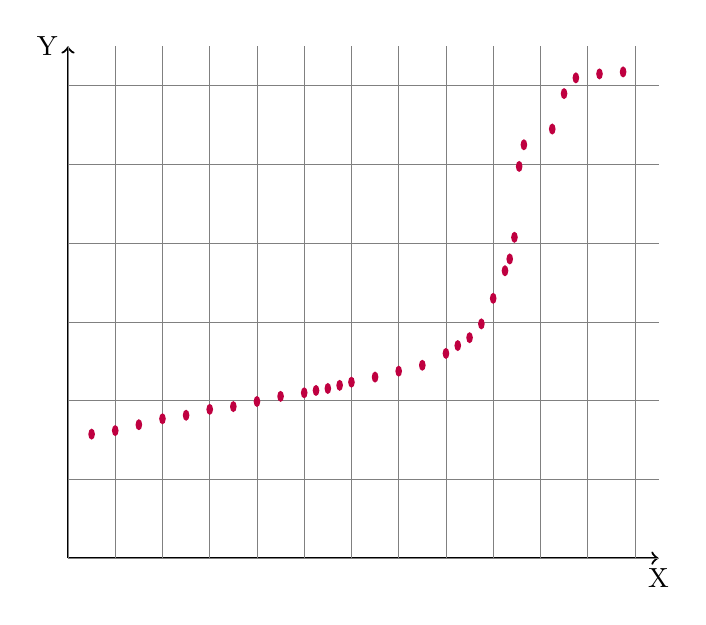
\begin{tikzpicture}[xscale = 0.3, yscale = 0.5]    
\draw[thick,->] (0,0) -- (25,0) node[anchor=north] {X};
\draw[thick,->] (0,0) -- (0,13) node[anchor=east] {Y};
\draw[gray, very thin](0,0) grid [step=2cm](25,13);
\fill[purple] (1,3.15) circle (4pt);
\fill[purple] (2,3.24) circle (4pt);
\fill[purple] (3, 3.39) circle (4pt);
\fill[purple] (4,3.54) circle (4pt);
\fill[purple] (5,3.63) circle (4pt);
\fill[purple] (6,3.78) circle (4pt);
\fill[purple] (7,3.85) circle (4pt);
\fill[purple] (8,3.98) circle (4pt);
\fill[purple] (9,4.11) circle (4pt);
\fill[purple] (10,4.2) circle (4pt);
\fill[purple] (10.5,4.26) circle (4pt);
\fill[purple] (11,4.31) circle (4pt);
\fill[purple] (11.5,4.39) circle (4pt);
\fill[purple] (12,4.47) circle (4pt);
\fill[purple] (13,4.6) circle (4pt);
\fill[purple] (14,4.75) circle (4pt);
\fill[purple] (15,4.9) circle (4pt);
\fill[purple] (16,5.2) circle (4pt);
\fill[purple] (16.5,5.4) circle (4pt);
\fill[purple] (17,5.6) circle (4pt);
\fill[purple] (17.5,5.95) circle (4pt);
\fill[purple] (18,6.6) circle (4pt);
\fill[purple] (18.5,7.3) circle (4pt);
\fill[purple] (18.7,7.6) circle (4pt);
\fill[purple] (18.9,8.15) circle (4pt);
\fill[purple] (19.1,9.95) circle (4pt);
\fill[purple] (19.3,10.5) circle (4pt);
\fill[purple] (20.5,10.9) circle (4pt);
\fill[purple] (21,11.8) circle (4pt);
\fill[purple] (21.5,12.2) circle (4pt);
\fill[purple] (22.5,12.3) circle (4pt);
\fill[purple] (23.5,12.35) circle (4pt);
\end{tikzpicture}

\caption{Titration Plot}

\end{figure}


% Note that IEEE does not put floats in the very first column - or typically
% anywhere on the first page for that matter. Also, in-text middle ("here")
% positioning is not used. Most IEEE journals use top floats exclusively.
% However, Computer Society journals sometimes do use bottom floats - bear
% this in mind when choosing appropriate optional arguments for the
% figure/table environments.
% Note that, LaTeX2e, unlike IEEE journals, places footnotes above bottom
% floats. This can be corrected via the \fnbelowfloat command of the
% stfloats package.
\subsection{Mathematics}
Now, Lets work on the Mathemetics symbols and formulas in LaTeX. Inorder to write mathematical formula and symbols, we need to use \verb|\usepackage{amsmath}| or \verb|\usepackage{mathrm}|. Here, inline \verb|$...$| will display equation in line. To display in centered of the page or column, we should put the formulas inside \verb|$$...$$|. To insert the fraction I can do \verb|\frac{}{}| where I can add the expressions inside the parenthesis. Here's an example using inline mode:
$\frac{n!}{k!(n-k)!} = \binom{n}{k}$. 

Here's an example of another mathematical expressions using display mode:
$$\frac{dy}{dx} = \lim_{\Delta x \to 0} \frac{f(x + \Delta x)-f(x)}{\Delta x}$$. Here, to write the delta symbol I used \verb|\Delta|. I have added the detailed explanation of this expression in \textbf{Appendix B}

Next, we can also add superscript and subscript in the expression by doing \verb|f^n| and \verb|f_{n}|. This will result in $f^n$ and $f_{n}$.Here's an example of univariate density function with subscripts and superscripts. Here, I used the product of univariate density functions:
\[ f_{n}(y;\theta) = \prod^n_{k=1} f^{univar}_{k}(y_{k}; 0)\]

\section{Conclusion}
Here, in this tutorial we started with creating simple document with title and now its ending with writing mathematical equations. I also wanted to give a detail overview of what is coming after conclusion in this document.
\begin{itemize}
    \item \verb|\appendices|- We can add Appendix section in the document by adding this command.
    \item \verb|\section*{Acknowledgements}| - This is how we can to add acknowledgements section in a document. 
    \item - Here, we have an example of how to add References in a document.
    \item \verb|\begin{thebibliography}| - This command will initiate to add the bibilography in the document. Don't forget to add the end to begin.
    \item \verb|\bibitem| - We also, have to be careful when adding the bibliographies in the document. Here, in bibliographies we use \verb|\bibitem| command.
\end{itemize}
I hope this tutorial was helpful.

%----- APPENDICES --------------------------------------------------------------------------------
\appendices
\section{}

Here in this appendix I am adding the extra commands that was not discussed in the tutorial.
\begin{enumerate}
    \item \verb|\textbf{}| - This command is used to make the text bold.
    \item \verb|\textit{}| - This command italicizes the text.
    \item \verb|\draw(n,n)(n,n)| - I used this command to draw the graph and set the dimensions, where n is replaced with the dimensions we want.
    \item \verb|\fill[color] (n,n) shape(npt)| - I used this command to fill the graph with all the titration points.
    \item \verb|\begin{enumerate}| - This helped me to set the environment and itemize with numbers
\end{enumerate}




% you can choose not to have a title for an appendix
% if you want by leaving the argument blank
\section{}
Here, I will go in detail about the mathematical expression I used. 

\begin{enumerate}
    \item \verb|\binom{}{}|- I used this function to write the binomial distribution formula.
    \item \verb|\lim_| - I used this command to write limit in the expression.
    \item \verb|\Delta| - This is a bit tricky. To get the triangular delta symbol we need to use Delta and the scientific delta symbol we use delta. So, be aware of the lower case and upper case D. 
    \item \verb|\theta| - I used this to add theta symbol in the document.
    \item \verb|\prod| - I used this to write that fancy symbol also called capital pi.
\end{enumerate}


%----- ACKNOWLEDGEMENT SECTION -------------------------------------------------------------------
% Explain what the asterisk * does in the next line: 
\section*{Acknowledgements}
I would like to thank Professor Moulds and the TAs for providing this opportunity to write this tutorial and help beginners to learn \LaTeX\. I has been truly a wonderful experience and I have learned new ways to use LaTeX which will definitely be very useful my future career. 


%----- BIBLIOGRAPHY ------------------------------------------------------------------------------

% You will need to explain how to include the bibliography section as follows. Explain the environment and how to add new items.
% Including how \ref, \cite and \label should be included here.

% Reminder: you will need to explain how to include the Bibliography Section and then include your own Bibliography at the end of your own tutorial.

\begin{thebibliography}{1}

\bibitem{IEEEhowto:kopka}
H.~Kopka and P.~W. Daly, \emph{A Guide to {\LaTeX}}, 3rd~ed.\hskip 1em plus
  0.5em minus 0.4em\relax Harlow, England: Addison-Wesley, 1999.

\bibitem{overleaf}
\text{Overleaf: https://www.overleaf.com/learn/latex/Tables}

\bibitem{LaTeX Math}
\text{LaTeX Math: https://en.wikibooks.org/wiki/LaTeX/Mathematics}


\end{thebibliography}

%----- Optional: BIOGRAPHY Section ---------------------------------------------------------------
 
% If you have an EPS/PDF photo (graphicx package needed) extra braces are
% needed around the contents of the optional argument to biography to prevent
% the LaTeX parser from getting confused when it sees the complicated
% \includegraphics command within an optional argument. (You could create
% your own custom macro containing the \includegraphics command to make things
% simpler here.)
%\begin{biography}[{\includegraphics[width=1in,height=1.25in,clip,keepaspectratio]{mshell}}]{Gerald Moulds}
% or if you just want to reserve a space for a photo:

%\begin{IEEEbiography}{Gerald Moulds}
%Biography text here.
%\end{IEEEbiography}

% if you will not have a photo at all:
%\begin{IEEEbiographynophoto}{John Doe}
%Biography text here.
%\end{IEEEbiographynophoto}

% insert where needed to balance the two columns on the last page with
% biographies
%\newpage

%\begin{IEEEbiographynophoto}{Jane Doe}
%Biography text here.
%\end{IEEEbiographynophoto}

% You can push biographies down or up by placing
% a \vfill before or after them. The appropriate
% use of \vfill depends on what kind of text is
% on the last page and whether or not the columns
% are being equalized.

%\vfill

% Can be used to pull up biographies so that the bottom of the last one
% is flush with the other column.
%\enlargethispage{-5in}

\end{document}
